 
 \section{Problem Statement} \label{Problem}

To date, the biggest experiment looking for proton decay signal is the Super-Kamiokande (SK) experiment \cite{SK}. SK is a big water tank containing 50 kton of ultra pure water located 1 km deep underground on a mine in the Japanese alps. When a charged particle travels at extremely high speeds inside the tank, it produces light, this is known as the Cherenkov effect \cite{Cherenkov}. In the walls of the tank there are photo-multiplier tubes (PMTs), which essentially are light detectors \cite{PMT}. Using these PMTs we know when a particle passed through the detector leaving a trace and producing light. In the SK tank there are more than 11 thousand PMTs to collect this light. We then have a data set with the time and charge of each PMT that received a hit. A reconstruction algorithm is then applied on this data so that physics quantities can be studied, like momentum, energy, direction and position of each particle that participated in the event.

As described in section \ref{Domain}, the proton decay mode that we are interested here consists of an anti-neutrino and a charged Kaon. The anti-neutrino has no electric charge, so it does not leave a trace in the detector and the Kaon also can not be seen, even though it has charge. That is because it does not have enough energy to be traveling at very high speeds, so it does not produce any light. But since the Kaon also decays, the hope is to see the decay products of the Kaon. Most of the time, it decays to a neutrino (which can not be seen) and an anti-muon\footnote{This is the only Kaon decay mode that will be used in the analysis here, but there is another decay mode that can be seen by SK.}, which is charged and has enough energy to be detected. Since this is a 2-body decay (the initial particle decays into 2 particles) and we know the masses of the final state particles, we also know the exact energy and momentum of the muon we are looking for (using energy and momentum conservation).

The problem is that after all this, the only visible particle that we can detect is the mono-energetic muon\footnote{This means that the energy of the muon is always the same. Also, since the SK can not detect the sign of the particle's charge (+ or -), we will not make a distinction between muons and anti-muons.}. This would make the search impossible, due to the amount of background events coming from atmospheric neutrino interactions. The solution is to look only for protons that decay inside the Oxygen nucleus of the water molecules, but not for the ones coming from the Hydrogen atoms. The difference is that when a proton decay inside the Oxygen, the remaining nucleus is left in an excited state and can emit a low energy photon (also called gamma) from nuclear de-excitation. If we look for this photon\footnote{The photon also does not have charge, but it produces electron-positron pairs as it travels in the water and these particles produce the Cherenkov light.} in coincidence with a mono-energetic muon, we then have a very particular signature in the detector that can be used to differentiate signal and background events. Figure \ref{fig:pdecay} shows a diagram of our final state particles.

\begin{figure}[h]
  \centering
  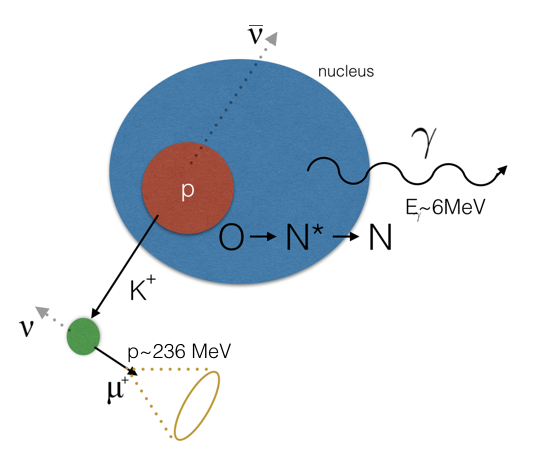
\includegraphics[width=0.37\linewidth]{figs/mugamma_mode.png}
  \caption{A proton inside an Oxygen nucleus decays to $\bar{\nu} + K^{+}$ and the remaining nucleus emits a 6 MeV photon. Later the Kaon decays into a $\nu$  and a mono-energetic  $\mu^{+}$ of about 236 MeV.}
  \label{fig:pdecay}
\end{figure}

Even though the situation is better now, it is still a challenge to identify if a signal comes from a proton that decayed or a neutrino that entered the detector and interacted with some nucleus. There are billions\footnote{Neutrinos come from many different sources, the main ones are the atmosphere and the Sun. Most of them cross our bodies, the Earth and all else and leave intact, since the chance of a neutrino interacting with something is incredibly small. Only from the Sun, 65 billion neutrinos cross a  person's thumb every second.} of neutrinos entering the detector every second. The chance of a neutrino interacting with a nucleus inside the tank is extremely small, but since the flux of incoming neutrinos is so high, we are bound to see some neutrino events\footnote{The detection of neutrinos in SK was awarded the Nobel prize in physics in 2015 for proving that neutrinos have mass \cite{Nobel}.} every hour or so.

Some of these events leave a trace in the detector that is very similar to our signal, so distinguishing between signal and background events is challenging. SK has searched for this decay mode before and the strategy used was to apply simple cuts in reconstructed variables such as momentum and number of particles present in the event. By looking at many distributions of these variables (features) and applying hard boundary cuts on them, a selection criteria was used to determine if an event is coming from signal or background. Details can be found here \cite{Miura}.

The rejection of background events is already very powerful in the standard analysis, however it would be better if it could be further improved. Due to the fact that proton decay was never observed, it is crucial to reduce number of False Positives as much as possible so that if an event is detected, we are confident that it comes from proton decay and not background. Even if no event is seen in the data, a lower limit for the proton lifetime can be calculated using a Poisson distribution. Increasing this limit is important to further restrict GUT models based on their predictions for the proton lifetime. This is how the first GUT based on the SU(5) model was rejected by Kamiokande data, a precursor of SK.

The goal of this study is to improve the selection criteria for this proton decay mode using Machine Learning techniques. This could enhance the signal-background separation leading to a better limit on the proton lifetime or ultimately the discovery of proton decay. This would be a huge discovery that will certainly change the current view of particle physics and deeper our knowledge of elementary particles and the fundamental interactions of nature. 
